\documentclass[a4paper, titlepage]{jsarticle}

\date{\today}
\usepackage[dvipdfmx]{graphicx}
\usepackage{url}
% \usepackage[T1]{fontenc}
\usepackage{float}
\usepackage{ascmac}
\usepackage{pdfpages}
\usepackage{enumitem}
\usepackage{otf}

\newcommand{\system}{\textsl{system name}}

\begin{document}
\begin{titlepage}
  \centering
  \vspace*{150truept}
  {\Large システム提案書}\\
  \vspace*{50truept}
  {\Huge ドローン宅配事業者支援システム} \\
  \vspace{15truept}
  {\Huge \system} \\
  \vspace{50truept}
  {\LARGE 土佐山田IT株式会社}\\
  \vspace{20truept}
  {\large{\tabcolsep = 1cm
      \begin{tabular}{ccc}
        久保田 天治 & 塩澤 康志 & 蝉 祐介  \\
        寺内 俊輔  & 林 晃太郎 & 松本 吏司
      \end{tabular}
    }}
\end{titlepage}

\tableofcontents

\clearpage

\section{現状の課題}
2022年日本における宅配便取扱個数は50億個を超えた.
忙しい日常がある中で,商品や郵便物を手軽に送受できる宅配便は多くの人々にとって頼りにされ,図\ref{fig:home_delivery}のように宅配需要は増加し続けている.
特に新型コロナウイルスの影響により,オンラインショッピングの増加や非接触配達の需要が高まり,宅配業界は一層の成長を遂げた.

しかし,宅配サービスの拡大と需要増加には新たな課題も浮かび上がっている,最も顕著な課題は宅配業界における労働力不足だ.
図\ref{fig:working_population}のように少子高齢化社会に伴う労働人口の減少により,現状の宅配サービスを維持することは日々困難になっている.
特に過疎地域や離島においては,現状の輸送方法では効率が悪く輸送方法の効率化が求められる.
\begin{figure}[H]
  \centering
  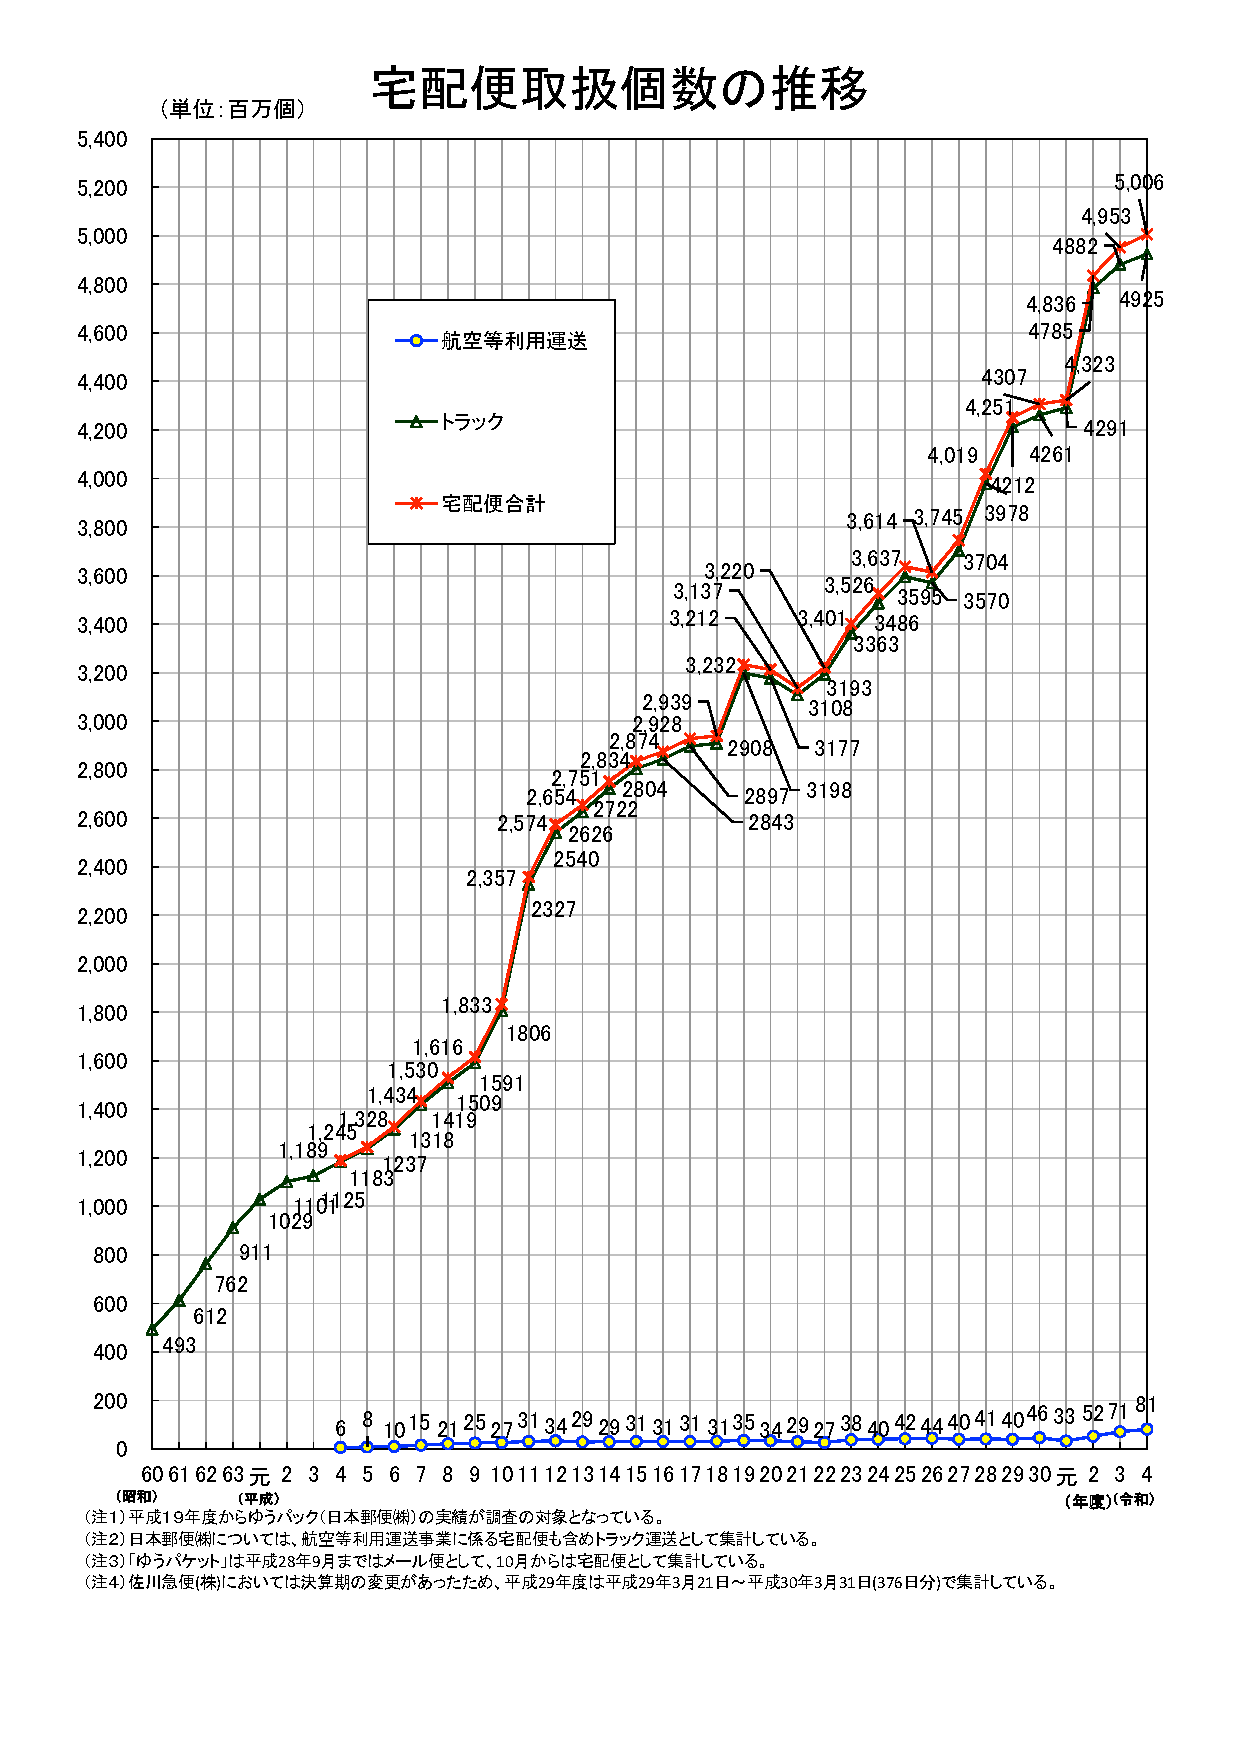
\includegraphics[width=0.6\textwidth]{./home_delivery.pdf}
  \caption{宅配便取扱個数の推移(\cite{home_delivery_2022}より引用)}
  \label{fig:home_delivery}
\end{figure}
\begin{figure}[H]
  \centering
  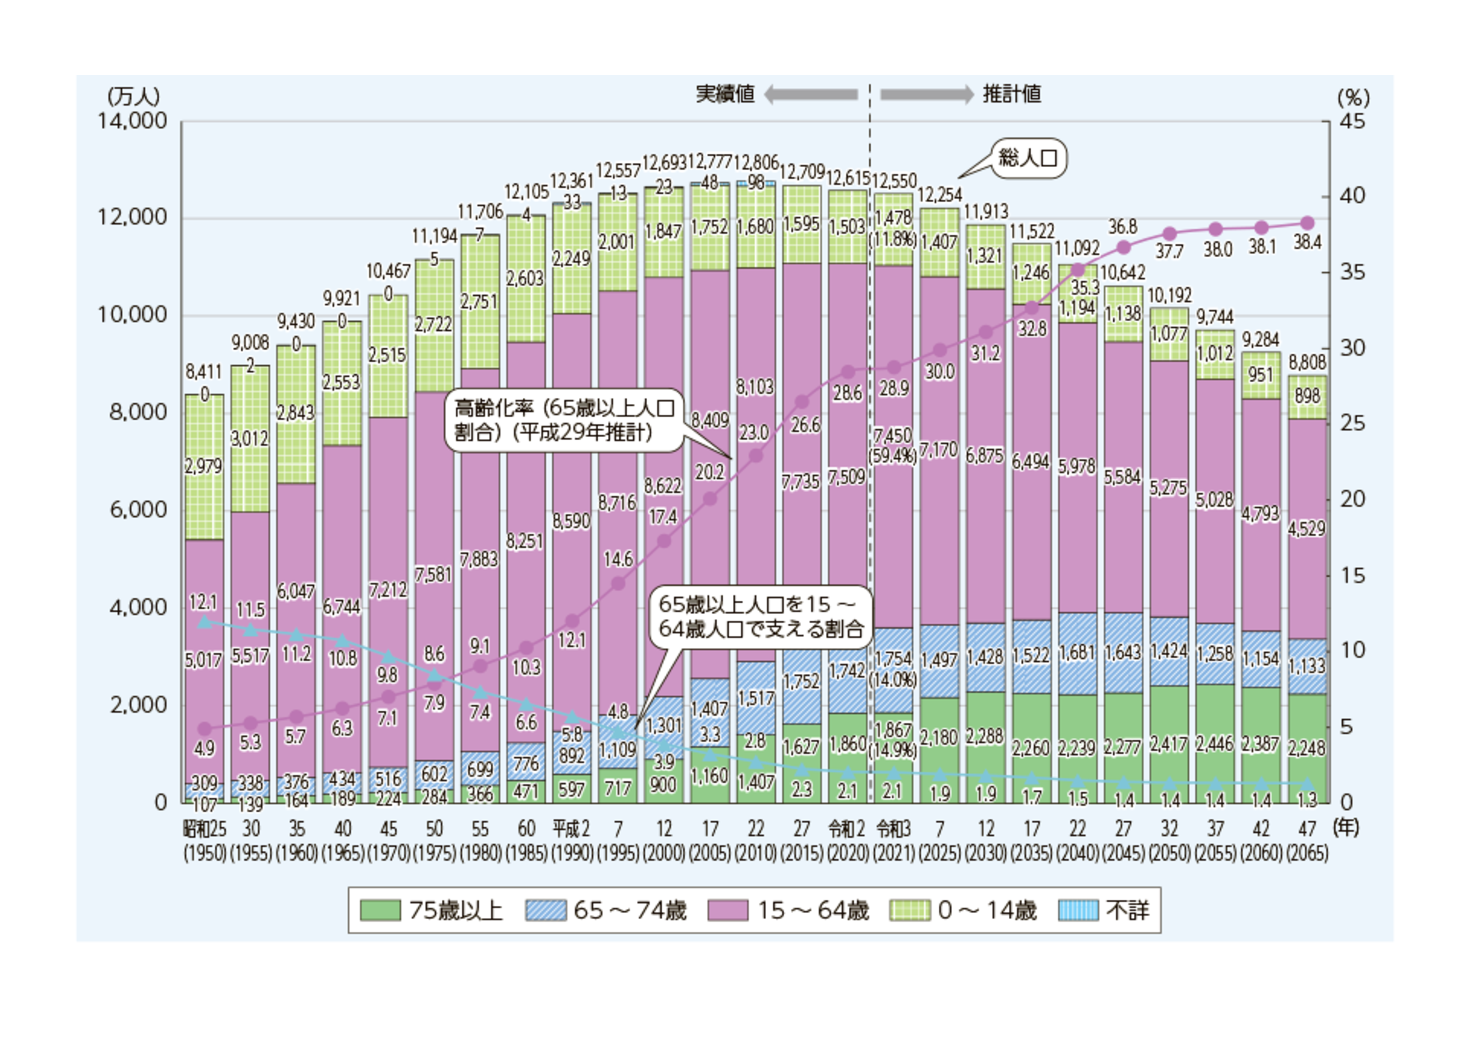
\includegraphics[width=0.8\textwidth]{./working_population.pdf}
  \caption{労働人口の減少(\cite{working_population_2022}より引用)}
  \label{fig:working_population}
\end{figure}

%名前
\section{課題解決のための提案}
上記の課題を解決するため,効率的かつ人手不足の解消を目的としたドローン宅配事業者支援システム"\system "を提案する.
このシステムによる課題の解決方法を以下に示す.
\begin{itemize}
  \item ドローンの操縦を自動化することで,より少ない人手で大量の荷物を個人宅に宅配でき,
        労働力不足の問題に対処できる.従来の宅配サービスと比較して労働者への依存度が低くなり,配送コスト削減と労働環境の改善に期待できる.
  \item 離島や過疎地域など従来の方法では非効率だった地域にも,効率的に配送を行うことができる.
        これによりこれらの地域においても高速かつ手頃な値段の宅配サービスが提供される.
\end{itemize}

\section{ドローン宅配の実現可能性}
\subsection{ドローンとは}
ドローンとは,リモートコントロールや事前にプログラムされた自律システムによって飛行する小型の航空機であり,一般的には無人航空機とも呼ばれる.

ドローンは,手のひらに収まるほどの小型機から,長時間の飛行が可能な大型機まで,様々な種類がある.これらのドローンは,サイズ・形状・機能・価格などが多様であり,カメラ・センサー・GPS・通信機能などの多彩な機能を備えたモデルが存在している.

\subsection{ドローンに関する法律}
現在のドローンに関する法律は次のようになっている.
\begin{quote}
  ドローン物流サービスの提供にあたっては、飛行の安全の確保の観点から、航空法第 11 章無人航空機に掲げる規定を遵守する必要がある。遵守されていない場合、航空法第 13 章罰則に掲げる規定により、罪に問われる場合がある。(\cite{delivery_guidelines_2023}より引用)
\end{quote}

現在,地表又は水面から150m以上の上空や人口集中地区などの,航空機の航行の安全に影響を及ぼすおそれのある空域や,落下した場合に地上の人などに危害を及ぼすおそれが高い空域において,ドローン等の無人航空機を飛行させるためには国土交通大臣の許可を得る必要がある.

無人航空機を飛行させるにあたり,次のルールを遵守する必要がある.\cite{prohibited_guidelines}
\begin{itemize}
  \item アルコールや薬物の影響下での運用を避けること.
  \item 飛行前に確認を行うこと.
  \item 他の航空機や無人航空機との衝突を防ぐための飛行を心掛けること.
  \item 他人に迷惑をかけるような方法での飛行を避けること.
\end{itemize}
また,特例を除き次に掲げる方法で無人航空機を飛行させる場合は,地方航空局長の承認を受ける必要がある.
\begin{itemize}
  \item 夜間での飛行.
  \item 目視外での飛行.
  \item 人または物件と距離を確保できない飛行.
  \item 催し場所上空での飛行.
  \item 危険物の輸送.
  \item 物資の投下.
\end{itemize}

ドローン宅配をするにあたり,人口集中地区で無人航空機を運用するためには,国土交通大臣の許可が必要である.また目視外の飛行を行うためには,地方航空局長の承認を得る必要がある.

\subsection{自動操縦について}
具体的な飛行について国土交通省や関連する機関が具体的なガイドラインや規定を定めており,飛行レベルは図\ref{fig:dron_level}のように定義されている.

\begin{figure}[htbp]
  \centering
  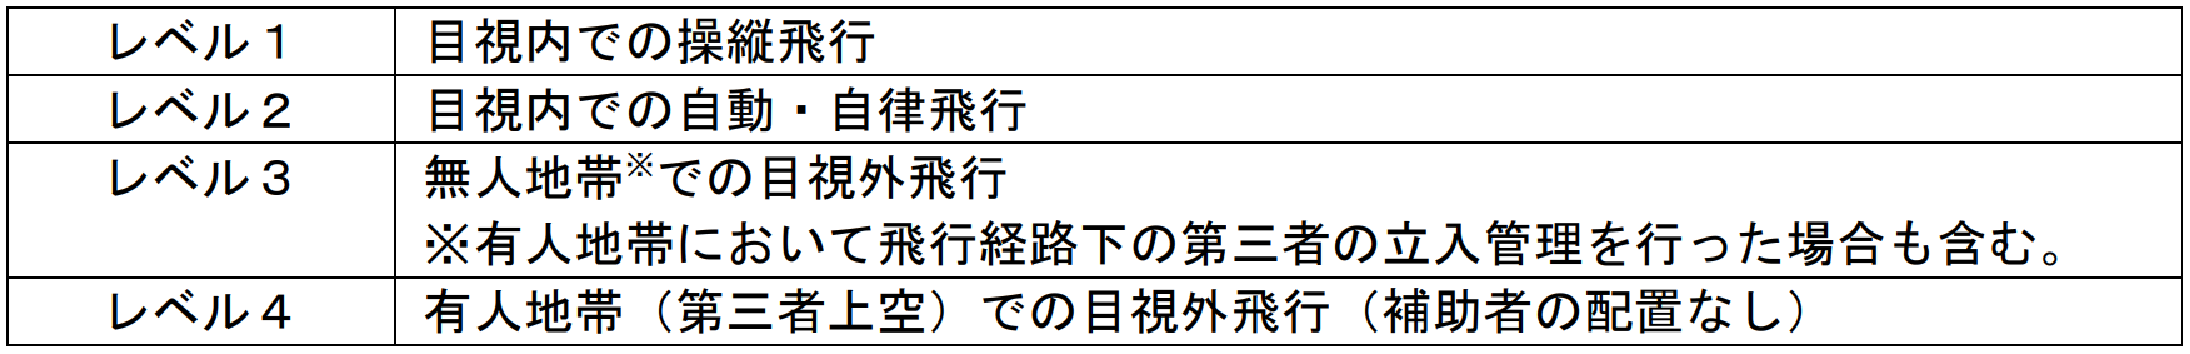
\includegraphics[width=0.8\textwidth]{flying_level.pdf}
  \caption{無人航空機の飛行レベル(\cite{delivery_guidelines_2023}より引用)}
  \label{fig:dron_level}
\end{figure}

ドローン宅配をするにあたり該当するレベルは,有人地帯での目視外飛行に該当するためレベル4である.

また,無人航空機の飛行形態や特定飛行の該非,立入管理措置の有無等により図\ref{fig:dron_category}のように3つのカテゴリーに分類される.
\begin{figure}[htbp]
  \centering
  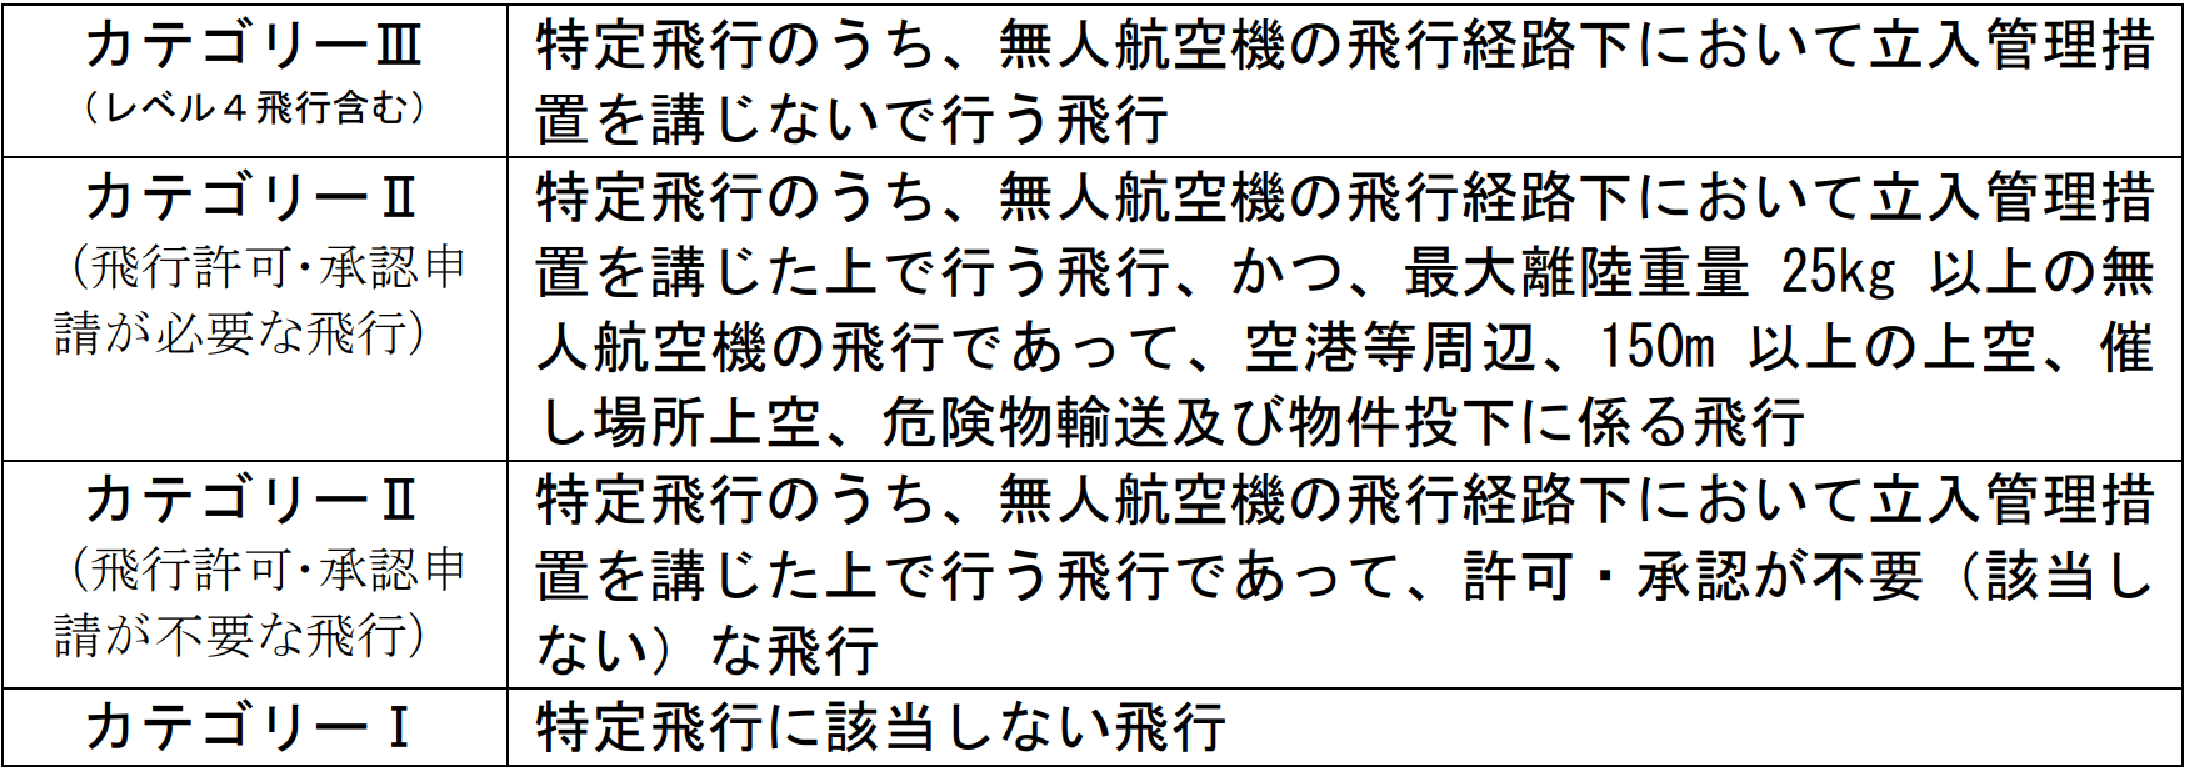
\includegraphics[width=0.8\textwidth]{dron_category.pdf}
  \caption{リスクに応じた無人航空機の飛行形態(\cite{delivery_guidelines_2023}より引用)}
  \label{fig:dron_category}
\end{figure}

無人航空機を飛行させるために必要な技能(知識及び能力)を有することを証明するため,無人航空機操縦者技能証明制度と呼ばれる制度が存在する.
%ローマ数字にする
カテゴリー\ajRoman{2}飛行を行うためには,二等無人航空機操縦士が必要であり,カテゴリー\ajRoman{3}飛行を行うためには,一等無人航空機操縦士が必要である\cite{delivery_guidelines_2023}.

\subsection{ドローン免許について}
\begin{table}[H]
  \centering
  \caption{ドローン免許(一等無人航空機操縦士)とトラック免許(準中型免許)の比較}
  \begin{tabular}{c c c} \hline
    免許     & 取得費用(円) & 取得条件  \\ \hline \hline
    ドローン免許 & 51800   & 16歳以上 \\
    トラック免許 & まだ      & 18歳以上 \\ \hline
  \end{tabular}
  \label{tab:hikaku}
\end{table}

%\subsection{労働力不足解消の可能性}
%近年,宅配サービスの拡大と需要増加にも関わらず,宅配業界の労働人口が不足している.労働人口の不足問題の解決方法の1つとして,ドローンの活用が考えられる.ドローン免許の国家資格としては,2022年12月5日から導入された.ドローン免許の一等無人航空機操縦士を取得することで,有人地帯(第三者上空)での目視外飛行(補助者の配置なし)が可能となった.受験資格は「16歳以上であること」,「航空法の規定により国土交通省から本試験の受験が停止されていないこと」となっており,免許受験費用については学科試験9,900円,実地試験22,000円,身体検査19,900円となっいることから,トラックの運転に必要な運転免許より少ない費用と期間でドローン免許を取得可能であることが期待できる.また,1人で複数台のドローンを飛ばすことができれば効率的に運ぶことができると考えられる.

%これらより,ドローン免許はトラックの免許の取得に必要な費用と期間を抑えることができるため,ドローンを活用することで労働力不足解消ができると考えられる.
% https://ua-remote-pilot-exam.com/certificate/
% https://ua-remote-pilot-exam.com/guide/eligibility/

\section{機能の概要・前提条件・制約事項}
\subsection{機能の概要}
本システムは管理者,ドローン宅配事業者,利用者が存在する.それぞれに向けた機能の概要を説明する.
ドローン宅配事業者は以下事業者と呼ぶ.
\subsubsection{管理者向け機能}
管理者用のwebページを作成し以下の機能を設ける.
%全部にする機能
\begin{description}[labelwidth=\linewidth]
  \setlength{\leftskip}{1em}
  \item [ログイン・ログアウト機能]管理者がログイン・ログアウトする機能.
  \item [事業者管理機能]事業者の登録情報の管理閲覧,絞り込み,請求書の送付,支払い状態の管理閲覧,貸与ドローンの管理閲覧.
  \item [利用者管理機能]利用者の登録情報の管理閲覧,絞り込み,請求書の送付,支払い状態の管理閲覧.
  \item [事業者情報分析機能]事業者の利用状況を絞り込みやグラフを用いて分析する機能.
  \item [利用者情報分析機能]利用者の利用状況を絞り込みやグラフを用いて分析する機能.
        %宅配依頼を受けることが
  \item [宅配依頼受付機能]利用者から宅配依頼を受け,受けることが可能か確認し,事業者に仕事を割り振ることが出来たら受付完了のフラグを返す機能.受付中,受付完了,集荷中,配送中,配送完了の状態を管理する.
        %まる
  \item [宅配仕事割り振り機能]宅配依頼受付機能で呼び出す,事業者に仕事を割り振る機能,集配に向かう事業者と仲介トラックと最終的に配送する事業者の組み合わせを選ぶ.
  \item [ドローン貸与機能]事業者からドローン貸与申請を受けて貸出あるいは,申請の差し戻しを行う機能.
  \item [事業者ドローン情報管理機能]事業者の所持ドローン,貸出用ドローンの登録,個数の変更,各ドローンの個体番号と稼働時間,各ドローンの状態閲覧を行う機能.
\end{description}

\subsubsection{事業者向け機能}
事業者用のwebページを作成し以下の機能を設ける.
\begin{description}[labelwidth=\linewidth]
  \setlength{\leftskip}{1em}
  \item [ログイン・ログアウト機能] 事業者用のログイン・ログアウトする機能.
  \item [事業者登録申請機能] 事業者名,事業代表者,免許情報,口座情報,事業拠点,従業員数,電話番号,メールアドレス,施設情報,パスワードを入力して事業者登録申請を行う機能.
  \item [事業者情報編集機能] 事業者名,事業代表者,免許情報,口座情報,事業拠点,従業員数,電話番号,メールアドレス,施設情報,パスワードを編集する機能.
  \item [依頼受注判断機能] 管理者から送られる宅配依頼を承諾もしくは拒否する機能.
  \item [配達完了通知機能] 宅配が完了した場合に利用者に通知する機能.
  \item [使用ドローン登録機能] 事業者が独自に購入したドローンを登録する機能.
  \item [子アカウント発行機能] 権限を限定した一般従業員用アカウントを発行して,同一事業者内で複数人が事業を行えるようにする機能.
  \item [子アカウント管理機能] 事業者が子アカウント発行機能を用いて発行した子アカウントの管理を行う機能.
  \item [ドローン貸与申請機能] ドローン貸与の申請,ドローンの返却,ドローンの修理依頼,ドローンの機体トラブル報告をする機能.
  \item [退会機能] 事業を終了し,データ削除を申請して退会する機能.
\end{description}

\subsubsection{利用者向け機能}
利用者向けのスマートフォン用ソフトウェアを用意し以下の機能を設ける.
\begin{description}[labelwidth=\linewidth]
  \setlength{\leftskip}{1em}
  \item [ログイン・ログアウト機能] 利用者用のログイン・ログアウトする機能.
        %登録情報を入れる
  \item [利用者会員登録機能] 利用者が会員登録をする機能,これは管理者の許可が必要ない.
  \item [宅配依頼機能] 管理者に対して宅配を依頼する機能.
  \item [受け取り完了通知機能] 受け取り完了を通知する機能.
  \item [宅配場所登録機能] 宅配で離着陸する場所を指定して登録する機能,外の画像を送信して申請をする.
  \item [お気に入り登録機能] 配送相手をお気に入り登録する機能,これを用いて簡単に宅配を依頼する機能.
  \item [退会機能] データ削除を申請して退会する機能.
\end{description}
\subsection{前提条件}
\begin{itemize}
  \item 宅配元と宅配先がお互いドローン着地地点を登録すること.
  \item 事業者は使用するドローンを無人航空機の登録制度に基づき国土交通省のシステムに登録すること.
  \item 宅配依頼に対し送り主と受け取り主の双方が同意すること.
  \item 利用者は日本語を理解できること.
\end{itemize}
\subsection{制約条件}
\begin{itemize}
  \item 利用者が情報を登録するときに虚偽の情報を登録しないこと.
  \item 管理者は利用者の情報を本システムの利用目的以外で使用しないこと.
  \item 管理者は利用者の個人情報の管理を情報漏洩のないように行うこと.
  \item 事業者は航空法施行規則236条に基づき無人航空機の適切な運用を行うこと.
  \item 荷物はW320$\times$D260$\times$H200(mm)以内に収まること\footnote{\label{fot:airtruck}物流専用ドローン AirTruck\cite{aeronext_airtruck}を想定}.
  \item 荷物は段ボールに梱包されていること.
  \item 荷物の重量は5kg以下であること\footref{fot:airtruck}.
  \item 利用者は利用規約を順守すること.
\end{itemize}
\section{ドローン宅配・情報・金銭の流れ}

\subsection{ドローン宅配の流れ}
本システムで想定するドローン宅配の流れを図\ref{fig:overview_flow}に示す.
また,以下に詳細な流れを示す.

\begin{enumerate}[label=\raise0.2ex\hbox{\textcircled{\scriptsize{\arabic*}}}]
  \item 送り主である利用者が,管理者に対して宅配依頼を行う.
  \item 管理者が事業者に対し,集荷・配送依頼を行う.
  \item 事業者がドローンを用い,依頼を受けた荷物の集荷を行う.
  \item 受け取り主である利用者が事業者から離れている場合,トラックを用いて荷物を受け取り主の最寄りの事業者へ配送する.
  \item 事業者がドローンを用い,荷物を受け取り主へ配達する.
\end{enumerate}

\begin{figure}[H]
  \centering
  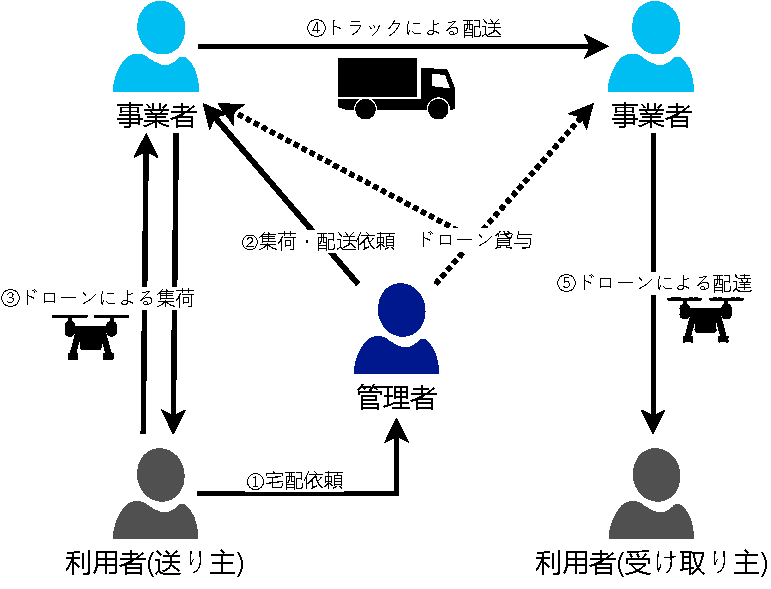
\includegraphics[width=0.6\linewidth]{./overview_flow.pdf}
  \caption{ドローン宅配の流れ}
  \label{fig:overview_flow}
\end{figure}

\subsection{情報の流れ}
本システムにおける情報の流れを図\ref{fig:info_flow}に示す.
本システムは,利用者(送り主及び受け取り主)が使用する端末,事業者が使用する端末,システム管理者が使用する端末及び,システム中核を担うサーバとデータベースによって構成される.

各ユーザからの要求を受けサーバが処理を行い,webページやソフトウェアに適した情報を提供する.

\begin{figure}[H]
  \centering
  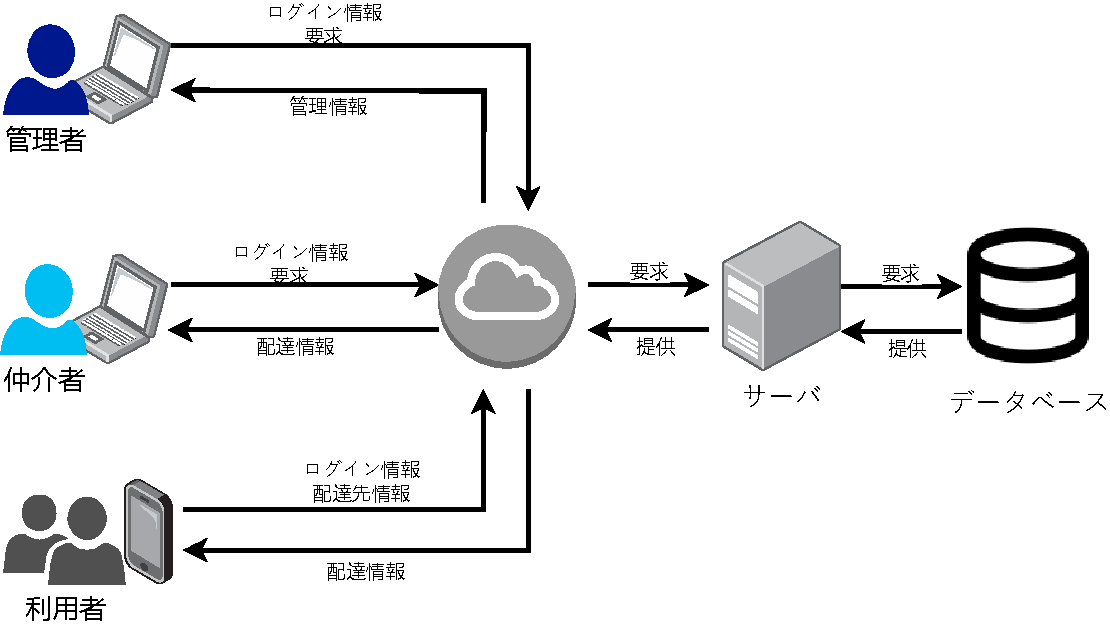
\includegraphics[width=0.8\linewidth]{./info_flow.pdf}
  \caption{本システムにおける情報の流れ}
  \label{fig:info_flow}
\end{figure}

\subsection{金銭の流れ}
本システムにおける金銭の流れを図\ref{fig:money_flow}に示す.

\begin{figure}[H]
  \centering
  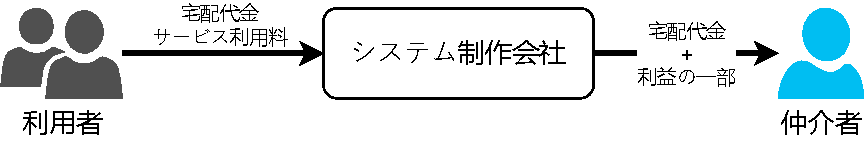
\includegraphics[width=0.8\linewidth]{./money_flow.pdf}
  \caption{本システムにおける金銭の流れ}
  \label{fig:money_flow}
\end{figure}


\section{想定する利用者}
本システムが想定する利用者を下記に示す.
\begin{itemize}
  \item 荷物の送受を希望する事業者または個人
  \item ドローン宅配事業者
\end{itemize}

\section{運用・保守}
\begin{itemize}
  \item 管理者がドローンを貸与する.
  \item システムは自社が運用保守を請け負う.
  \item 事業者は管理者にドローンの修理依頼をする.
  \item 管理者は専門の業者にドローンの修理依頼を出す.
  \item 最低月に1度ミーティングと修正を行う.
  \item システムのアップデートを行う.
  \item 管理者からの不具合等の対応はメールで対応し,営業時間内で対応する.
\end{itemize}

\section{ハードウェア・ソフトウェアの構成}
\subsection{ハードウェア構成}
本システムのハードウェア構成を表\ref{fig:hardware}に示す.
\begin{table}[H]
  \begin{center}
    \caption{ハードウェアの構成}
    \label{fig:hardware}
    \begin{tabular}{ccc} \hline
      項目        & 種類      & 数量       \\ \hline \hline
      メインサーバ    & レンタルサーバ & 2        \\
      データベースサーバ & レンタルサーバ & 2        \\
      管理者端末     & PC      & 1        \\
      事業者端末     & PC      & 事業者数     \\
      利用者端末     & スマートフォン & 利用者数     \\
      搬送装置      & ドローン    & 事業者希望数以上 \\ \hline
    \end{tabular}
  \end{center}
\end{table}
\subsection{ソフトウェア構成}
本システムのソフトウェア構成を表\ref{fig:software}に示す.
\begin{table}[H]
  \begin{center}
    \caption{ソフトウェアの構成}
    \label{fig:software}
    \begin{tabular}{ccc} \hline
      項目    & ソフトウェア          & 備考 \\ \hline \hline
      サーバ   & ApacheもしくはNginx &    \\
      サーバ   & DBMS            &    \\
      サーバ   & ドローン管理システム      &    \\
      管理者端末 & 管理者用システム        &    \\
      事業者端末 & 事業者用システム        &    \\
      利用者端末 & 利用者用システム        &    \\ \hline
    \end{tabular}
  \end{center}
\end{table}

\section{費用・効果}
\subsection{システムの効果}
本システムを導入することによって,以下の効果が期待できる.
\begin{itemize}
  \item ドローンを用いた無人宅配が可能となり,宅配サービスの人手不足を解消できる.
  \item ドローンを用いて処方薬を配送することで,山間部や離島などに対するリモート診療に利用できる.
  \item ドローンを用いたフードデリバリーといった新たなサービスが提供でき,経済の活性化につながる.
  \item 充電式のドローンを使用することで,排気ガスの排出が削減され,環境への負荷が軽減する.
        そのため,環境への配慮を重視する現代社会に貢献できる.
  \item 管理者が多くの事業者にサービスを提供することで,新規ドローン宅配事業者の参入を奨励できる.
        新規事業者の参入に伴う宅配業務従事者の増加と競争の活発化は,労働力不足の解消,サービス品質の向上,価格競争力の向上につながり,消費者にとって選択肢が増えることで市場が活性化する.
  \item 多くの事業者が共通の支援システムを使用することで,スケールメリットを最大限に活用しコスト削減を実現できる.
        経済的なメリットは宅配業界全体に波及し,より効率的なサービス提供が可能になる.
\end{itemize}

\subsection{収益}
%0.14%の話をフッターに書く,本文には20000個と書く
本システムの収益は配達による収入を想定している.配送料を600円,1日に配達する荷物の数を20,000個\footnote{\label{fot:baggage}宅配便の1日当たりの荷物数の約0.14\%}とすると5年間の配達による収入は

\begin{center}
  600円$\times$20,000個$\times$30日$\times$60ヶ月=21,600,000,000円
\end{center}
となる.

\subsection{システムの導入・運用コスト}
本システムの導入コストは表\ref{tab:label1},運用コストは表\ref{tab:label2}のようになる.
%ドローンの個数を10倍,備考に参考にしたドローンを記載
\begin{table}[H]
  \centering
  \caption{導入コスト}
  \begin{tabular}{c c c c c}
    \hline
    項目          & 単価(千円) & 数量            & 金額(千円)    & 備考                                           \\
    \hline \hline
    物流ドローン(貸出用) & 3,000  & 2,000台        & 6,000,000 & 物流専用ドローン AirTruck\cite{aeronext_airtruck}を参考 \\
    サーバ(レンタル)   & 2      & 4ヶ月$\times$2台 & 16        &                                              \\
    システム設計人件費   & 40     & 34日$\times$6人 & 8,160     &                                              \\
    システム実装人件費   & 40     & 31日$\times$6人 & 7,440     &                                              \\
    \hline \hline
                & 合計     &               & 6,015,616 &                                              \\
    \hline
  \end{tabular}
  \label{tab:label1}
\end{table}

\begin{table}[H]
  \centering
  \caption{運用コスト}
  \begin{tabular}{c c c c c}
    \hline
    項目        & 単価(千円)    & 数量                             & 金額(千円)     & 備考                             \\
    \hline \hline
    サーバ(レンタル) & 2         & 60ヶ月$\times$2台                 & 240        & 変動の可能性あり                       \\
    維持費用      & 6,015,616 & 60ヶ月                           & 3,007,808  & (導入コスト$\times$10\% )$\times$5年 \\
    宅配事業者報酬   & 0.15      & 20,000個$\times$30日$\times$60ヶ月 & 5,400,000  & 報酬$\times$1日当たりの荷物の数$\times$日数 \\
    中間配送費用    & 35        & 40台$\times$30日$\times$60ヶ月     & 2,520,000  & トラック1台の報酬$\times$台数$\times$日数  \\
    \hline \hline
              & 合計        &                                & 10,928,048 &                                \\
    \hline
  \end{tabular}
  \label{tab:label2}
\end{table}

上記を踏まえて,システムの開発と5年間の運用にかかる費用は次のようになる.
\begin{center}
  6,015,616,000円(導入コスト)+10,928,048,000円(運用コスト)=16,943,664,000円
\end{center}

\subsection{利益}
本システムを5年間運用した際の利益は以下のようになる.
\begin{center}
  21,600,000,000円(収益)-16,943,664,000円(費用)=4,656,336,000円
\end{center}

\section{開発体制と工程計画}
本システムの開発は土佐山田IT株式会社の6名により行う.

本システムの工程計画は図\ref{fig:schedule}に示す.
%1月1日みたいにする
\begin{figure}[H]
  \centering
  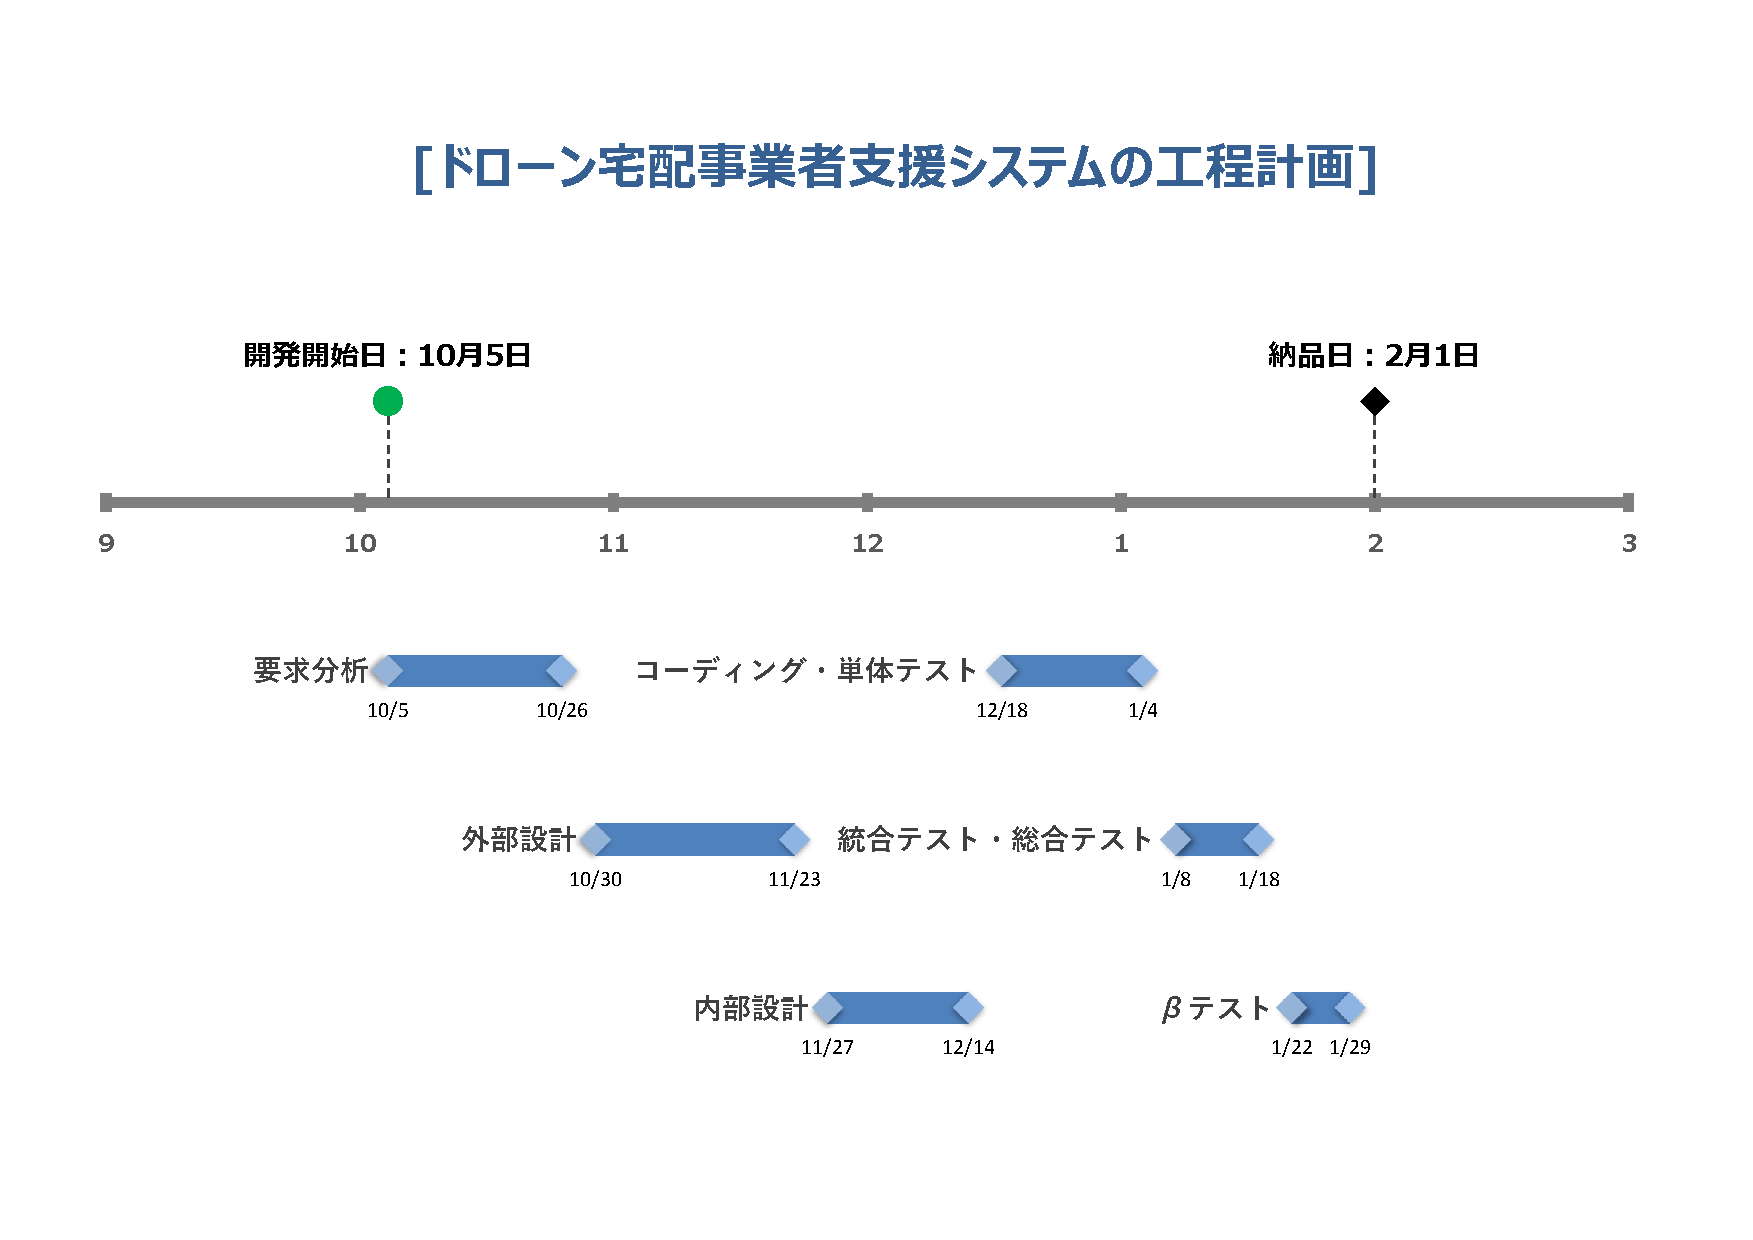
\includegraphics[width=0.8\textwidth]{schedule.pdf}
  \caption{工程計画}
  \label{fig:schedule}
\end{figure}

\section{本システムのアピールポイント}
\begin{itemize}
  \item 未だに日本に存在のしないシステムである.
  \item 2022年度の宅配荷物数は50億個であり,8年連続史上最高を更新中である.しかし,人手不足が深刻化しており,本システムはこの課題の解決策のひとつとなりうる.
  \item 交通渋滞や地理的な制約を受けずに荷物を迅速かつ効率的に配達することが可能である.
  \item 災害時などで交通インフラが破壊されたとしても,物理的障害の影響が少ないため,必要な物資や医療用品の迅速な配達が可能である.
  \item 離島や山間部などのアクセスが難しい地域において従来の宅配方法と比較し,大幅なコスト削減になる.
  \item 今日リモート診療が普及し始めている.リモート診療とドローン宅配を併用すると患者は外出する必要がなくなるため,感染リスクを極力減らすことができる.
\end{itemize}

\section{貢献度}
システム提案書では各メンバーが以下の項目でチームに貢献した.
\begin{itemize}
  \item 1240312 久保田 天治
        \begin{itemize}
          \item 機能の概要・前提条件・制約事項一部
          \item ハードウェアとソフトウェアの構成
          \item 制約の追加と語句の修正と語句表の作成
          \item レビューの司会
          \item レビュの際に積極的に改善点を提示
        \end{itemize}
  \item 1250329 塩澤 康志
        \begin{itemize}
          \item 費用・効果
          \item システム導入の効果の追加
        \end{itemize}
  \item 1250333 蝉 祐介
        \begin{itemize}
          \item 運用・保守
          \item 労働力不足解消の可能性を追加
          \item 10/16(月)の会議で書記を担当
        \end{itemize}
  \item 1250348 寺内 俊輔
        \begin{itemize}
          \item 機能の概要・前提条件・制約事項一部
          \item 現状の課題
          \item 課題解決のための提案
          \item 全体の枠組み
          \item 全体の統合
          \item 機能の概要追加
          \item 「労働力不足の可能性の追加」と「ドローン宅配の実現の可能性」について個別ミーティング
          \item 参考文献の収集と提示
          \item チームメンバーのサポート
          \item 購入用ドローンの選定
          \item レビュの際に積極的に改善点を提示
        \end{itemize}
  \item 1250358 林 晃太郎
        \begin{itemize}
          \item 想定する利用者
          \item スケジュール
          \item 本システムのアピールポイント
          \item 3回の会議で書記を担当
          \item 10/16の会議の体調不良者に代わりリーダーを担当
          \item 会議のリーダーを4回担当(リーダー代行も含め)
          \item ドローンの実現可能性のsectionを追加
          \item 工程計画の作成
          \item 購入用ドローンの申請
          \item レビュの際に積極的に改善点を提示
        \end{itemize}
  \item 1250371 松本 吏司
        \begin{itemize}
          \item 情報・金銭の流れ
          \item 全体の枠組み
          \item Githubにおけるルール整備・リポジトリ整備・コマンド共有
          \item Slackにgithub bot導入
          \item ドローン宅配の流れの図作成
          \item 分かれた文書の統合
          \item レビュの際に積極的に改善点を提示
        \end{itemize}
\end{itemize}
%できればURLの前に改行
\bibliography{References.bib}
\bibliographystyle{plain}


\end{document}
